\section{第 10 章综合习题}

\begin{problem}{符号函数二重积分}{Sgn-Double-Integral}
    计算二重积分 $I = \iint_{D} \operatorname{sgn}(x^2 - y^2 + 2) \d x \d y$，其中 $D = \{(x, y) : x^2 + y^2 \le 4\}$。
\end{problem}

\begin{solution}
    根据符号函数的定义，令 $D_1 = \{(x, y) \in D : x^2 - y^2 + 2 \ge 0\}$，$D_2 = \{(x, y) \in D : x^2 - y^2 + 2 < 0\}$。则有
    \begin{equation}
        I = \iint_{D_1} 1 \d A - \iint_{D_2} 1 \d A = \operatorname{Area}(D_1) - \operatorname{Area}(D_2).
    \end{equation}
    由于 $\operatorname{Area}(D_1) + \operatorname{Area}(D_2) = \operatorname{Area}(D) = 4\uppi$，故
    \begin{equation}
        I = 4\uppi - 2\operatorname{Area}(D_2).
    \end{equation}
    区域 $D_2$ 由双曲线 $y^2 - x^2 = 2$ 在圆 $x^2 + y^2 = 4$ 内部的部分组成。联立方程
    \begin{equation}
        \begin{cases}
            x^2 + y^2 = 4, \\
            y^2 - x^2 = 2.
        \end{cases} \implies y^2 = 3, \ x^2 = 1.
    \end{equation}
    交点为 $(\pm 1, \pm \sqrt{3})$。$D_2$ 包含上下两个对称部分，其面积为
    \begin{equation}
        \operatorname{Area}(D_2) = 2 \int_{-1}^1 \left( \sqrt{4-x^2} - \sqrt{x^2+2} \right) \d x.
    \end{equation}
    分别计算其中的积分：
    \begin{equation}
        \begin{aligned}
            \int_{-1}^1 \sqrt{4-x^2} \d x & = \left[ \frac{x}{2}\sqrt{4-x^2} + 2\arcsin \frac{x}{2} \right]_{-1}^1 = \sqrt{3} + \frac{2\uppi}{3}, \\
            \int_{-1}^1 \sqrt{x^2+2} \d x & = \left[ \frac{x}{2}\sqrt{x^2+2} + \ln(x + \sqrt{x^2+2}) \right]_{-1}^1 = \sqrt{3} + \ln(2+\sqrt{3}).
        \end{aligned}
    \end{equation}
    从而得到
    \begin{equation}
        \operatorname{Area}(D_2) = 2 \left( \frac{2\uppi}{3} - \ln(2+\sqrt{3}) \right) = \frac{4\uppi}{3} - 2\ln(2+\sqrt{3}).
    \end{equation}
    代入 $I$ 的表达式：
    \begin{equation}
        I = 4\uppi - 2 \left( \frac{4\uppi}{3} - 2\ln(2+\sqrt{3}) \right) = \frac{4\uppi}{3} + 4\ln(2+\sqrt{3}).
    \end{equation}

    \begin{center}
        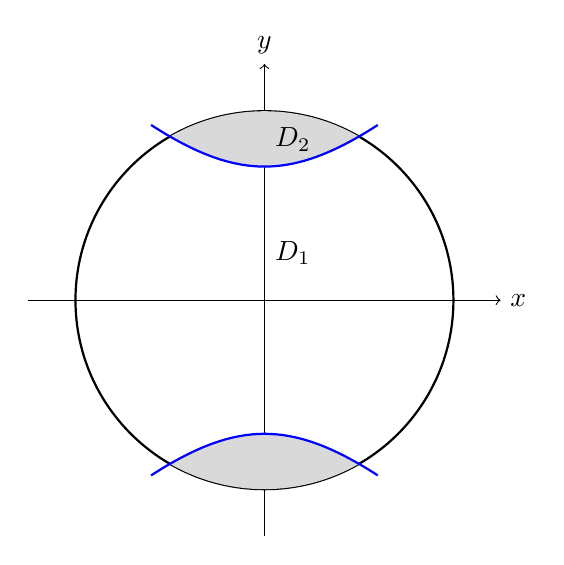
\begin{tikzpicture}[scale=1.2]
            \draw[->] (-2.5,0) -- (2.5,0) node[right] {$x$};
            \draw[->] (0,-2.5) -- (0,2.5) node[above] {$y$};
            \draw[thick] (0,0) circle (2);
            \fill[gray!30, domain=-1:1, samples=50]
            plot (\x, {sqrt(\x*\x+2)}) -- plot[domain=1:-1] (\x, {sqrt(4-\x*\x)}) -- cycle;
            \fill[gray!30, domain=-1:1, samples=50]
            plot (\x, {-sqrt(\x*\x+2)}) -- plot[domain=1:-1] (\x, {-sqrt(4-\x*\x)}) -- cycle;
            \draw[thick, blue, domain=-1.2:1.2, samples=50] plot (\x, {sqrt(\x*\x+2)});
            \draw[thick, blue, domain=-1.2:1.2, samples=50] plot (\x, {-sqrt(\x*\x+2)});
            \node at (0.3, 1.7) {$D_2$};
            \node at (0.3, 0.5) {$D_1$};
        \end{tikzpicture}
    \end{center}

    \begin{equation}
        \boxed{I = \frac{4\uppi}{3} + 4\ln(2+\sqrt{3})}
    \end{equation}
\end{solution}

\begin{problem}{三重积分}{Triple-Integral-Unit-Cube}
    计算三重积分
    \begin{equation}
        I = \iiint_{[0,1]^3} \frac{\d u \d v \d w}{(1 + u^2 + v^2 + w^2)^2}.
    \end{equation}
\end{problem}

\begin{solution}
    \ansitem{1}

    利用积分恒等式 $\frac{1}{A^2} = \int_0^\infty t \e^{-At} \d t$，将原积分表示为
    \begin{equation}
        \begin{aligned}
            I & = \iiint_{[0,1]^3} \left( \int_0^\infty t \e^{-(1 + u^2 + v^2 + w^2)t} \d t \right) \d u \d v \d w                                                      \\
              & = \int_0^\infty t \e^{-t} \left( \int_0^1 \e^{-tu^2} \d u \right) \left( \int_0^1 \e^{-tv^2} \d v \right) \left( \int_0^1 \e^{-tw^2} \d w \right) \d t.
        \end{aligned}
    \end{equation}

    令 $f(t) = \int_0^1 \e^{-tx^2} \d x$，则有
    \begin{equation}
        I = \int_0^\infty t \e^{-t} f(t)^3 \d t.
    \end{equation}

    通过分部积分可建立 $f(t)$ 与 $\e^{-t}$ 的关系
    \begin{equation}
        f(t) = \left[ x \e^{-tx^2} \right]_0^1 - \int_0^1 x (-2tx) \e^{-tx^2} \d x = \e^{-t} + 2t \int_0^1 x^2 \e^{-tx^2} \d x = \e^{-t} - 2t f'(t).
    \end{equation}

    整理得 $\e^{-t} = f(t) + 2t f'(t)$，代入 $I$ 的表达式
    \begin{equation}
        \begin{aligned}
            I & = \int_0^\infty t \left( f(t) + 2t f'(t) \right) f(t)^3 \d t                \\
              & = \int_0^\infty \left( t f(t)^4 + 2t^2 f(t)^3 f'(t) \right) \d t            \\
              & = \int_0^\infty \frac{\d}{\d t} \left( \frac{1}{2} t^2 f(t)^4 \right) \d t.
        \end{aligned}
    \end{equation}

    考察边界值。当 $t \to 0$ 时，显然 $t^2 f(t)^4 \to 0$；当 $t \to \infty$ 时，利用高斯积分的渐近性质
    \begin{equation}
        f(t) \sim \int_0^\infty \e^{-tx^2} \d x = \frac{\sqrt{\uppi}}{2\sqrt{t}},
    \end{equation}

    可得极限值
    \begin{equation}
        \lim_{t \to \infty} t^2 f(t)^4 = \lim_{t \to \infty} t^2 \left( \frac{\uppi}{4t} \right)^2 = \frac{\uppi^2}{16}.
    \end{equation}

    综上所述，积分结果为
    \begin{equation}
        \boxed{I = \frac{\uppi^2}{32}}
    \end{equation}
\end{solution}





\endinput
